
\begin{figure}[h]        
    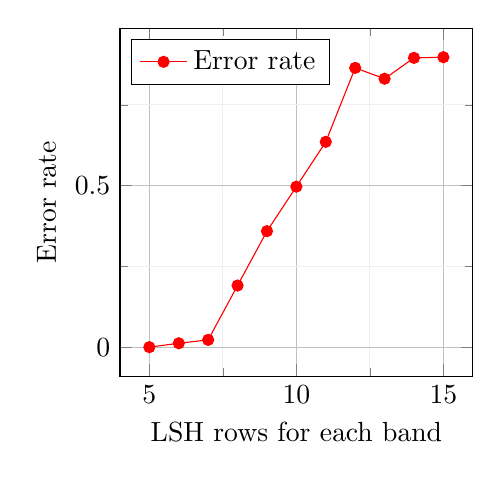
\begin{tikzpicture}
    \begin{axis}[
        xlabel=LSH rows for each band,
        ylabel=Error rate,
        height=6cm,
        width = 0.5*\textwidth,
        grid = both,
        minor tick num = 1,
        major grid style = {lightgray},
        minor grid style = {lightgray!25},
        legend cell align = {left},
        legend pos = north west
    ]
    
    \addplot[color=red,mark=*] coordinates {
        (5, 0.001)
        (6, 0.013)
        (7, 0.023499)
        (8, 0.1915)
        (9, 0.3595)
        (10, 0.497)
        (11, 0.6355)
        (12, 0.864)
        (13, 0.8305)
        (14, 0.895)
        (15, 0.897)
    };
    
    
    \legend{Error rate}
    \end{axis}
    \end{tikzpicture}
    
    \caption{\normalfont As the size of each band rises, the error rate increases.}
    \label{fig:rows_per_band_error_rate}
\end{figure}
